\documentclass[11pt]{article}
\usepackage[letterpaper,margin=1in]{geometry}
\usepackage{graphicx}
\usepackage{amsmath}
\usepackage{amssymb}
\usepackage{xcolor}
\usepackage{booktabs}
\usepackage{tikz-cd}
\usepackage{hyperref}
\usepackage[numbers,sort&compress]{natbib}
\usepackage{titlesec}
\titlespacing*{\section}{0pt}{1.5ex plus 1ex minus .2ex}{1ex plus .2ex}
\hypersetup{colorlinks=true,linkcolor=blue,urlcolor=blue,citecolor=blue}
\bibliographystyle{unsrtnat}

\def\LAOSTO{LaAlO$_3$/SrTiO$_3$}
\newcommand{\cellname}[1]{\texttt{#1}}
\tikzcdset{every label/.append style={font=\scriptsize}}

\title{Rebuilding a published figure from raw acquisitions with Yoneda}
\author{}
\date{}

\begin{document}
\maketitle
\vspace{-4em}

\section{What was done}

We took one published figure, Fig.~2 of Briggeman \textit{et al.}~\cite{Briggeman2025-pk}, and rebuilt it from the raw files the acquisition software wrote in 2017. The figure shows the four-terminal conductance and transconductance of a chiral superlattice written at the \LAOSTO{} interface and of a straight control waveguide on the same device, at 25~mK and fields up to 18~T. Every step from the raw bytes to the finished image passes through a Yoneda instance, and the figure is computed from the instance by query. The data deposit that accompanies the paper~\cite{Briggeman2025-data} was not used to make the figure. It was read once, at the end, to compare.

The work was done by an AI agent in a single session, from a short request, and the audited figure existed within 45 minutes of it. The agent located the raw data on the laboratory drive by the sample tag, read undocumented instrument headers, identified which of two conflicting channel assignments was correct, matched runs to figure panels, recovered the calibration, and identified two processing steps between the raw files and the published panels that the files do not record. Every one of those judgments entered the instance as a claim carrying its evidence, so each can be checked or retracted without touching the data. Figure~\ref{fig:compare} shows the result. A rebuild from raw bytes takes 25~s, and redrawing from the instance alone reproduces the image byte for byte.

\begin{figure}[h]
\centering
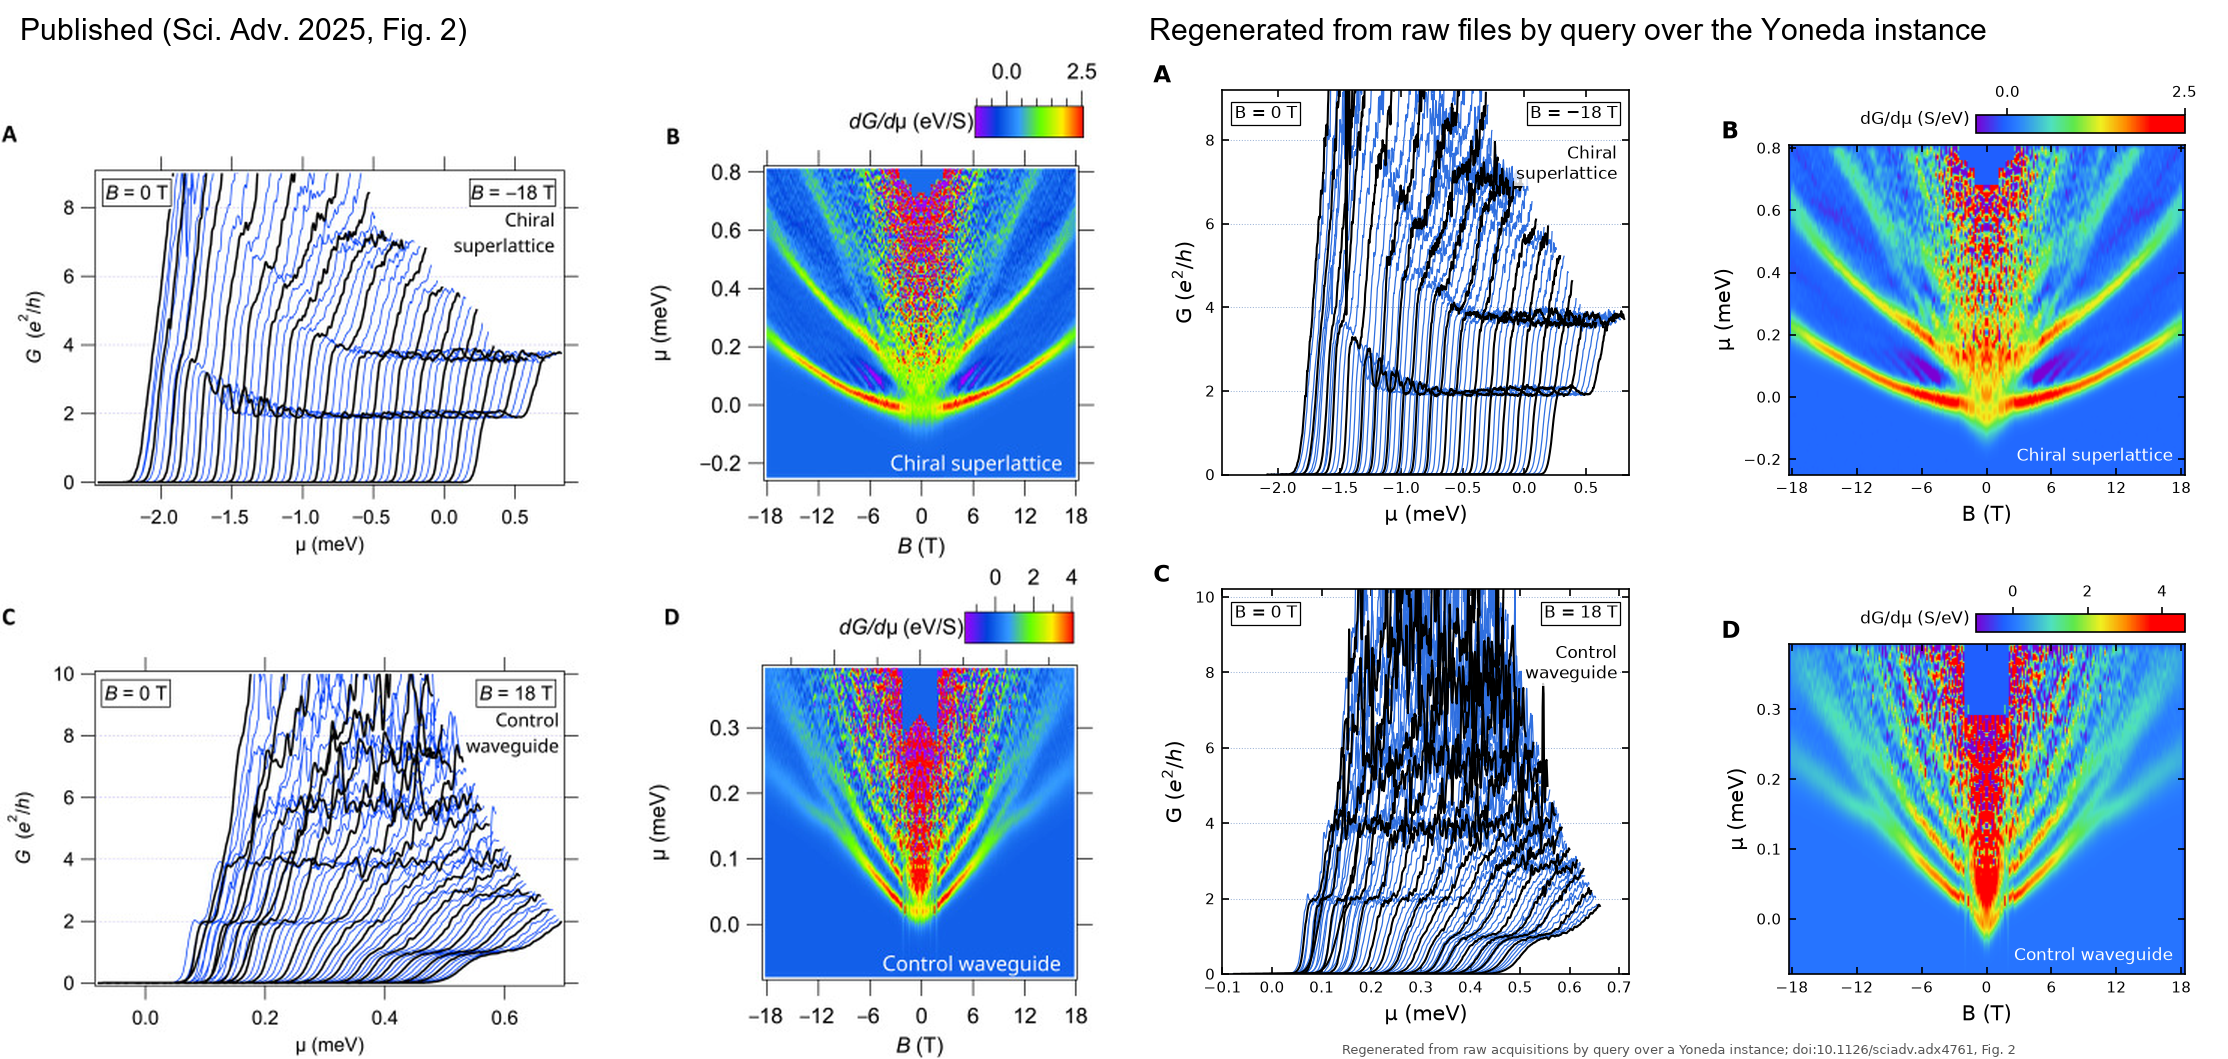
\includegraphics[width=\textwidth]{fig/yoneda-fig2-side-by-side.png}
\caption{Left, Fig.~2 as published~\cite{Briggeman2025-pk} (CC BY 4.0). Right, the same four panels computed by query over the Yoneda instance from 237 raw gate sweeps (66~MB) in two runs of one cooldown. Panels A and C are conductance waterfalls, B and D transconductance maps. The maps agree with the published ones at correlation 0.985 (superlattice) and 0.892 (control) for $|B|>3$~T. Below about 2~T the two differ where the published maps were aligned by a rule that is not recorded (Section~4).}
\label{fig:compare}
\end{figure}

\section{Ingest: save first, name by fingerprint, connect later}

The single store is the laboratory data tree, cooldown folder \texttt{MNK/SA03018F.20171127}, which holds 19,331 files from 59 experiments. Every file enters as a cell whose identity is the SHA-256 of its bytes. A \cellname{located} cell records where those bytes were found, and nothing is copied out of the store. Each acquisition file becomes a \cellname{run} cell with two times, the event time read from the file's own clock (2 December 2017) and the record time at which the instance wrote it (18 October 2026). A run has faces pointing at its file and its experiment. Whole-folder ingest took one pass and did not change the figure, because the figure asks the instance which runs to use.

Meaning then accrues as claims. Each file states its wiring twice, once in a lock-in table typed into the header and once in an index block written by the acquisition software. Both enter as \cellname{wiring} claims. Each is checked against the conductance the instrument itself computed during the measurement, which is stored in the same file. The typed table reproduces it to 0.1\% in every run. In two of three runs the software's index block still lists the wiring of the other section of the device, and misses by factors of 1470 and 17,980. Those two claims are retracted by \cellname{outcome} cells whose faces point at the claim and at the failed check. The retracted claims stay in the instance with their author and date. The view \cellname{active} no longer returns them, so no computation sees them. Figure~\ref{fig:tower} shows the cells involved.

\begin{figure}[h]
\centering
\vspace{1em}
\begin{tikzcd}[column sep=3.6em, row sep=3em, cells={nodes={font=\small}}]
\text{file} & \text{run} \ar[l, "\mathsf{file}"'] \ar[d, "\mathsf{experiment}"'] & |[draw, dashed, inner sep=4pt]| \text{wiring} \ar[l, "\mathsf{evidence}"'] \ar[dl, "\mathsf{experiment}"] & \text{check} \ar[l, "\mathsf{of}"'] & \text{outcome} \ar[l, "\mathsf{because}"'] \ar[ll, bend right=40, "\mathsf{of}"'] \\
& \text{experiment} & & &
\end{tikzcd}
\caption{One correction, as stored. Each arrow points from a cell to one of its faces, labeled by role. Reading the top row from left to right, each cell sits one level above the cells it points at: file (level 0), run (1), wiring claim (2), check (3), outcome (4). The file and experiment cells are named by their content; the others are authored, with an instance and two times. The dashed wiring claim is retracted by the outcome cell. It remains in the instance and is excluded by the \cellname{active} view. Adding the correction added two cells and no table.}
\label{fig:tower}
\end{figure}

A further set of claims connects the runs to the paper. A \cellname{depicts} claim links each panel to a run, with the experimenter's own processed file for that section of the device as evidence. A \cellname{lever-arm} claim carries the calibration $\mu = \mu_0 + \alpha V_{sg}$, read off the published axes against the raw gate range ($\alpha = 8.13~\mu$eV/mV for the superlattice and $3.93~\mu$eV/mV for the control), with the published image itself entered as a file cell and named as evidence.

\section{Rebuilding the figure}

Each step of the arithmetic is a \cellname{derivation} cell. Its faces are its inputs, the code that ran (named by the hash of the source file) and its output, and its data are its parameters. The output is stored as a blob named by its own hash. For the superlattice the chain is conductance from the active wiring claim, removal of discrete gate jumps, smoothing and differentiation with mirror symmetrization in field, and the figure. The jump removal follows one stated rule and records what it found, three jumps of 5.8, 3.2 and 6.7~mV at $-2.28$, $-1.48$ and $-0.83$~T. The figure cell names 13 witnesses: the paper, the four panel claims, the lever-arm claims and the derivations that supplied the arrays.

Verification is a statement that a diagram commutes (Fig.~\ref{fig:ladder}). The top row is the arithmetic, rerun from the raw bytes. Each vertical arrow is the hash function $h$, which turns content into a name. The bottom row is what the instance stored, derivation cells relating one name to the next. The audit recomputes every step from the inputs and parameters its cell names and checks $h(\text{recomputed output}) = \text{recorded name}$. All squares commuted, for two builds made from scratch and again after the instance was moved to another folder. All 237 raw files were re-hashed on every read and matched their cells.

\begin{figure}[h]
\centering
\begin{tikzcd}[column sep=2.5em, row sep=3em, cells={nodes={font=\small}}]
\text{raw sweeps} \ar[r, "G"] \ar[d, "h"'] & G(B, V_{sg}) \ar[r, "U"] \ar[d, "h"] & G_{\text{aligned}} \ar[r, "T"] \ar[d, "h"] & \partial G/\partial V_{sg} \ar[r, "F"] \ar[d, "h"] & \text{figure} \ar[d, "h"] \\
\text{file ids} \ar[r, "d_G"'] & \texttt{715570da} \ar[r, "d_U"'] & \texttt{30e22f43} \ar[r, "d_T"'] & \texttt{b972aadf} \ar[r, "d_F"'] & \texttt{748312408c}
\end{tikzcd}
\caption{The rebuild as a ladder of commuting squares, for panel B. Top, the computation: conductance $G$, jump removal $U$, transconductance $T$, rendering $F$. Down, SHA-256. Bottom, the derivation cells stored in the instance, with the leading hex digits of each output name. Commutation of every square is the audit. Because names are functions of content, two independent builds produce the same names, and two copies of an instance merge as a union on identity with nothing to remap.}
\label{fig:ladder}
\end{figure}

\section{Comparing with the published figure}

Read against the deposit, the published waterfall curves are the raw sweeps shifted uniformly in gate voltage, by 1.50~mV for the superlattice and 0.75~mV for the control, to within 0.15~mV at every field. After that shift they agree with the raw sweeps to 0.05~$e^2/h$ (median, $|B|>4$~T). The size fits a correction for lock-in lag at this sweep rate. The files do not record it, so the rebuilt figure plots the sweeps as recorded.

This comparison has a natural categorical form (Fig.~\ref{fig:natural}). Let the field sweep be a category whose objects are the field values and whose morphisms are steps along the sweep, and let $R$ and $P$ assign to each field the raw and the published curve. A processing step that is the same at every field is a natural transformation $\eta: R \Rightarrow P$, and the waterfall shift is one: its component $\eta_B$ is translation by 1.50~mV for every $B$, so each naturality square commutes. For the maps, our aligned rows $U$ and the published rows $M$ are related by a constant shift for $|B|>3$~T and by no single shift below about 1.5~T, where the two alignment rules differ. The squares fail exactly there. A failure of naturality locates a processing step that depends on where in the measurement it was applied. Steps of that kind are usually done by hand.

\begin{figure}[h]
\centering
\begin{tikzcd}[column sep=3em, row sep=2.6em, cells={nodes={font=\small}}]
R(B) \ar[r] \ar[d, "\eta_B"'] & R(B') \ar[d, "\eta_{B'}"] \\
P(B) \ar[r] & P(B')
\end{tikzcd}
\hspace{5em}
\begin{tikzcd}[column sep=3em, row sep=2.6em, cells={nodes={font=\small}}]
U(B) \ar[r] \ar[d, dashed, "?"'] & U(B') \ar[d, dashed, "?"] \\
M(B) \ar[r] & M(B')
\end{tikzcd}
\caption{Left, the published waterfall differs from the raw sweeps by a natural transformation, a shift of $+1.50$~mV in $V_{sg}$ at every field, and every square commutes. Right, the published map and ours agree for $|B|>3$~T and the squares fail below about 1.5~T, where the gate-jump alignment differs.}
\label{fig:natural}
\end{figure}

\section{What the categorical structure provides}

\paragraph{One table at every order of statement.} A file, a run, a claim about the run, a check of the claim and the retraction of the claim are the same kind of row, a cell whose faces point at other cells. The correction in Fig.~\ref{fig:tower} sits four levels above the data and required no new table. A schema that separates nodes from edges stores the first two levels and needs a new table at the third. Disagreement between two sources, here a typed header and a machine-written index, is stored the way any other statement is stored, and the view \cellname{active} applies at every level unchanged.

\paragraph{Meaning by relation.} The Yoneda lemma states that an object is determined by its morphisms into it~\cite{MacLane1998-cwm,Riehl2016-context}. A run here has no description beyond its bytes. What it means is the set of cells that point at it, which the library returns as $\mathrm{Hom}(-,X)$, and that set grows as interpretation accumulates without any earlier cell being rewritten. The figure is the clearest case, an object whose content is the list of its 13 witnesses.

\paragraph{Identity is a function of content.} Hashing sends equal content to equal names on any machine~\cite{Benet2014-ipfs}. A reader can check any file or derived array by recomputing its name. A recomputation is verified by comparing names, which is the audit in Fig.~\ref{fig:ladder}. Copies of an instance merge as a union on identity. Authored claims get time-ordered identifiers and carry their author, so independent claims about the same bytes stay distinct.

\paragraph{Provenance is composition.} Each derivation is a morphism from named inputs to a named output, and the figure is their composite. Asking where a pixel came from is following arrows back to raw files, with the code and parameters of each step on the way, in the form the W3C provenance model describes~\cite{Moreau2013-provdm}. Because the figure is computed from active claims, retracting a claim changes the figure with no change to code, and the old figure remains with its own witnesses.

\paragraph{Naturality as a test.} Comparing a reconstruction with a publication becomes a question about squares (Fig.~\ref{fig:natural}). Where they commute the published processing was a convention applied uniformly, and it can be stated as one parameter. Where they fail, the difference is located in the measurement, at specific fields, and can be raised with the people who did the work. Across a corpus this gives a way to count the unrecorded steps between the instrument and the page, field by field and laboratory by laboratory. Functorial treatments of data migration~\cite{Spivak2012-fdm,Fong2019-sevensketches} provide the general setting.

\paragraph{AI as an auditable participant.} Every judgment the agent made here (which wiring is correct, which run is in which panel, what the calibration is, where the jumps are) entered as a claim with named evidence, and every computation as a derivation that can be rerun. The agent's work can therefore be checked step by step by a person or by another agent, and any step can be retracted without losing the rest.

\section{Availability}

The reconstruction is public at \texttt{github.com/levylabpitt/yoneda-reconstruction}. It contains the code, the instance (2.7~MB), its derived arrays (4.5~MB) and a marimo notebook that redraws the figure, shows the cells described here, and reruns the audit when the raw files are mounted. The Yoneda genome is included as a submodule at the commit the instance records, and the repository is laid out to take further reconstructions, one folder per figure.

\bibliography{yoneda-reconstruction}

\end{document}
